% ----------------------------------------------------------
% Tecnologias Envolvidas
% ----------------------------------------------------------
\chapter{Arquitetura e Modelagem do Sistema} \label{cha:arquitetura}

\section{Arquitetura da Solução}
Esta seção descreve a organização estrutural do sistema BusLy, que provê funções de gestão de transporte para empresas: cadastro de empresas, usuários, motoristas, veículos, rotas, paradas, viagens e bilhetes. A solução adota uma arquitetura web em camadas, com separação clara entre apresentação (frontend), lógica de negócio e APIs (backend) e persistência (banco de dados).

No \textit{frontend}, utiliza-se Next.js~15 com roteamento via App Router, estado de sessão via NextAuth (estratégia \textit{JWT}) e componentes React tipados (TypeScript). O \textit{frontend} consome APIs REST autenticadas, mantém contexto de usuário/empresa e incorpora mapas e edição geográfica com Leaflet/React-Leaflet para operações sobre rotas e paradas.

O \textit{backend} é implementado com NestJS~11, estruturado por módulos de domínio (\textit{auth}, \textit{users}, \textit{companies}, \textit{drivers}, \textit{vehicles}, \textit{stops}, \textit{routes}, \textit{trips}, \textit{tickets}, etc.). As regras de negócio são expostas por controladores REST, protegidos por autenticação \textit{JWT} e autorização baseada em papéis. A multiempresa é tratada por \textit{companyId} e por um interceptor que injeta o contexto de empresa a partir do token. A persistência usa TypeORM com PostgreSQL.

\begin{figure}[H]
\centering
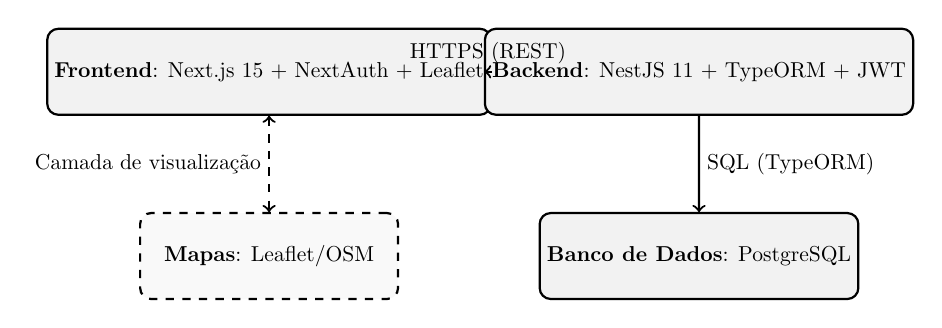
\begin{tikzpicture}[scale=0.78, every node/.style={transform shape}]
  \tikzumlset{font=\footnotesize}
  % Blocos
  \node[draw, rounded corners, thick, fill=gray!10, minimum width=4.2cm, minimum height=1.4cm, align=center] (fe) at (0,0) {\textbf{Frontend}: Next.js 15 + NextAuth + Leaflet};
  \node[draw, rounded corners, thick, fill=gray!10, minimum width=4.8cm, minimum height=1.4cm, align=center] (be) at (7,0) {\textbf{Backend}: NestJS 11 + TypeORM + JWT};
  \node[draw, rounded corners, thick, fill=gray!10, minimum width=4.2cm, minimum height=1.4cm, align=center] (db) at (7,-3) {\textbf{Banco de Dados}: PostgreSQL};
  \node[draw, dashed, rounded corners, thick, fill=gray!5, minimum width=4.2cm, minimum height=1.4cm, align=center] (maps) at (0,-3) {\textbf{Mapas}: Leaflet/OSM};

  % Conexões
  \draw[->, thick] (fe) -- node[above]{HTTPS (REST)} (be);
  \draw[->, thick] (be) -- node[right]{SQL (TypeORM)} (db);
  \draw[<->, thick, dashed] (fe) -- node[left]{Camada de visualização} (maps);
\end{tikzpicture}
\caption{Visão de alto nível da solução.}
\end{figure}

\section{Modelagem do Banco de Dados}
O modelo de dados foi projetado para refletir as agregações de negócio. A Tabela~\ref{tab:principais-entidades} sumariza as principais entidades e seus papéis. De forma geral, todas as entidades operacionais são associadas a uma empresa (\textit{multi-tenancy} por chave estrangeira \texttt{company\_id}). Rotas possuem paradas ordenadas (\texttt{route\_stops}) e agenda de operação (\texttt{route\_schedules}); viagens instanciam rotas em horários específicos e originam bilhetes.

\begin{table}[H]
\centering
\begin{tabular}{ll}
\toprule
\textbf{Entidade} & \textbf{Descrição resumida} \\
\midrule
\texttt{companies} & Empresa (razão social, nome fantasia, CNPJ, slug, contato) \\
\texttt{users} & Usuário (nome, e-mail, senha, papel, status, \texttt{company\_id}) \\
\texttt{drivers} & Motorista (CPF, CNH, categoria, status, \texttt{company\_id}) \\
\texttt{vehicles} & Veículo (placa, capacidade, categoria, status, \texttt{company\_id}) \\
\texttt{addresses} & Endereço (CEP, logradouro, geocoordenadas) \\
\texttt{stops} & Parada (nome, \texttt{address\_id}, acessibilidade, \texttt{company\_id}) \\
\texttt{routes} & Rota (nome, distância, duração estimada, \texttt{company\_id}) \\
\texttt{route\_stops} & Associação rota–parada com ordem e horário opcional \\
\texttt{route\_schedules} & Agenda por dia da semana para a rota \\
\texttt{trips} & Viagem (rota, janelas horárias, status, assentos, \texttt{company\_id}) \\
\texttt{tickets} & Bilhete (passageiro, preço, assento, pontos de embarque) \\
\bottomrule
\end{tabular}
\caption{Principais entidades do domínio.}
\label{tab:principais-entidades}
\end{table}

O diagrama de classes da Figura~\ref{fig:uml-dominio} sintetiza os relacionamentos mais relevantes do domínio.

\begin{figure}[H]
\centering
\begin{tikzpicture}[scale=0.35, every node/.style={transform shape}]
  \tikzumlset{font=\tiny}
  
  % NÍVEL 1: Empresa (topo da hierarquia)
  \umlclass[x=18,y=25]{Company}{
    id: uuid\\
    legalName: string\\
    tradeName: string\\
    slug: string\\
    cnpj: string\\
    email: string\\
    phone: string\\
    logoUrl: string\\
    createdAt: Date\\
    updatedAt: Date
  }{ }
  
  % NÍVEL 2: Gestão de usuários e recursos
  \umlclass[x=3,y=18]{User}{
    id: uuid\\
    name: string\\
    email: string\\
    phone: string\\
    photoUrl: string\\
    password: string\\
    role: UserRole\\
    status: UserStatus\\
    companyId: uuid\\
    createdAt: Date\\
    updatedAt: Date
  }{ }
  
  \umlclass[x=18,y=18]{Vehicle}{
    id: uuid\\
    plate: string\\
    model: string\\
    brand: string\\
    year: number\\
    capacity: number\\
    category: VehicleCategory\\
    comfortConfiguration: ComfortConfiguration\\
    busType: BusType\\
    acquisitionDate: Date\\
    odometer: number\\
    lastMaintenance: Date\\
    nextMaintenance: Date\\
    status: VehicleStatus\\
    notes: string\\
    companyId: uuid
  }{ }
  
  \umlclass[x=33,y=18]{Driver}{
    id: uuid\\
    name: string\\
    cpf: string\\
    licenseNumber: string\\
    licenseCategory: string\\
    licenseExpiry: Date\\
    phone: string\\
    email: string\\
    birthDate: Date\\
    hireDate: Date\\
    status: DriverStatus\\
    emergencyContactName: string\\
    emergencyContactPhone: string\\
    address: string\\
    notes: string\\
    companyId: uuid
  }{ }
  
  % NÍVEL 3: Configuração de rotas
  \umlclass[x=8,y=11]{Route}{
    id: uuid\\
    name: string\\
    description: string\\
    isActive: boolean\\
    estimatedDuration: string\\
    distance: number\\
    companyId: uuid
  }{ }
  
  \umlclass[x=23,y=11]{Stop}{
    id: uuid\\
    name: string\\
    addressId: uuid\\
    isActive: boolean\\
    hasAccessibility: boolean\\
    hasShelter: boolean\\
    companyId: uuid
  }{ }
  
  \umlclass[x=38,y=11]{Address}{
    id: uuid\\
    cep: string\\
    street: string\\
    number: string\\
    complement: string\\
    neighborhood: string\\
    city: string\\
    state: string\\
    longitude: number\\
    latitude: number\\
    createdAt: Date\\
    updatedAt: Date
  }{ }
  
  % NÍVEL 4: Relacionamentos de configuração
  \umlclass[x=8,y=4]{RouteSchedule}{
    id: uuid\\
    routeId: uuid\\
    dayOfWeek: number\\
    isActive: boolean\\
    createdAt: Date\\
    updatedAt: Date
  }{ }
  
  \umlclass[x=23,y=4]{RouteStop}{
    id: uuid\\
    routeId: uuid\\
    stopId: uuid\\
    order: number\\
    departureTime: string
  }{ }
  
  % NÍVEL 5: Operação - Viagens
  \umlclass[x=3,y=-3]{TripVehicle}{
    id: uuid\\
    tripId: uuid\\
    vehicleId: uuid\\
    primaryDriverId: uuid\\
    secondaryDriverId: uuid\\
    isActive: boolean\\
    observations: string\\
    createdAt: Date\\
    updatedAt: Date
  }{ }
  
  \umlclass[x=18,y=-3]{Trip}{
    id: uuid\\
    routeId: uuid\\
    departureTime: Date\\
    estimatedArrivalTime: Date\\
    actualDepartureTime: Date\\
    actualArrivalTime: Date\\
    status: TripStatus\\
    basePrice: number\\
    totalSeats: number\\
    availableSeats: number\\
    isAutoGenerated: boolean\\
    observations: string\\
    companyId: uuid\\
    createdAt: Date\\
    updatedAt: Date
  }{ }
  
  % NÍVEL 6: Vendas - Bilhetes
  \umlclass[x=33,y=-3]{Ticket}{
    id: uuid\\
    tripId: uuid\\
    passengerName: string\\
    passengerDocument: string\\
    passengerPhone: string\\
    passengerEmail: string\\
    seatNumber: string\\
    price: number\\
    status: TicketStatus\\
    boardingPointType: BoardingPointType\\
    boardingStopId: uuid\\
    boardingLocationDescription: string\\
    boardingLatitude: number\\
    boardingLongitude: number\\
    landingPointType: BoardingPointType\\
    landingStopId: uuid\\
    landingLocationDescription: string\\
    landingLatitude: number\\
    landingLongitude: number\\
    observations: string\\
    companyId: uuid
  }{ }

  % RELACIONAMENTOS HIERÁRQUICOS PRINCIPAIS
  % Company -> Recursos
  \umlassoc[mult1=1,mult2=*,pos1=0.05,pos2=0.95]{Company}{User}
  \umlassoc[mult1=1,mult2=*,pos1=0.05,pos2=0.95]{Company}{Vehicle}
  \umlassoc[mult1=1,mult2=*,pos1=0.05,pos2=0.95]{Company}{Driver}
  
  % Company -> Configuração
  \umlassoc[mult1=1,mult2=*,pos1=0.05,pos2=0.95,arm1=-135,arm2=90]{Company}{Route}
  \umlassoc[mult1=1,mult2=*,pos1=0.05,pos2=0.95,arm1=-45,arm2=90]{Company}{Stop}
  
  % Configuração de endereços
  \umlassoc[mult1=1,mult2=*,pos1=0.05,pos2=0.95]{Address}{Stop}
  
  % FLUXO PRINCIPAL: Route -> RouteStop <- Stop
  \umlassoc[mult1=1,mult2=*,pos1=0.05,pos2=0.95]{Route}{RouteStop}
  \umlassoc[mult1=1,mult2=*,pos1=0.05,pos2=0.95]{Stop}{RouteStop}
  
  % Horários das rotas
  \umlassoc[mult1=1,mult2=*,pos1=0.05,pos2=0.95]{Route}{RouteSchedule}
  
  % FLUXO OPERACIONAL: Route -> Trip
  \umlassoc[mult1=1,mult2=*,pos1=0.05,pos2=0.95]{Route}{Trip}
  \umlassoc[mult1=1,mult2=*,pos1=0.05,pos2=0.95,arm1=-135,arm2=90]{Company}{Trip}
  
  % Trip -> TripVehicle (associação veículo/motorista)
  \umlassoc[mult1=1,mult2=*,pos1=0.05,pos2=0.95]{Trip}{TripVehicle}
  \umlassoc[mult1=1,mult2=*,pos1=0.05,pos2=0.95,arm1=-90,arm2=90]{Vehicle}{TripVehicle}
  \umlassoc[mult1=1,mult2=*,pos1=0.05,pos2=0.95,arm1=-90,arm2=135,stereo=<<primaryDriver>>]{Driver}{TripVehicle}
  
  % Relacionamentos de TripVehicle
  \umlassoc[mult1=1,mult2=*,arm1=-90,arm2=90]{Vehicle}{TripVehicle}
  \umlassoc[mult1=1,mult2=*,stereo=<<primaryDriver>>]{Driver}{TripVehicle}
  
  % Relacionamento opcional: Stop -> Ticket (embarque/desembarque específico)
  \umldep[stereo=<<boarding/landing>>,mult1=0..1,mult2=*,pos1=0.05,pos2=0.95,arm1=-90,arm2=135]{Stop}{Ticket}
  
\end{tikzpicture}
\caption{Diagrama de classes detalhado do domínio BusLy.}
\label{fig:uml-dominio}
\end{figure}

\subsection{Diagramas UML Fracionados por Agregado}
Para facilitar a leitura, os diagramas a seguir detalham os principais agregados do domínio.

\subsubsection*{Agregado Organizacional: Empresas e Usuários}
\begin{figure}[H]
\centering
\begin{tikzpicture}[scale=0.9, every node/.style={transform shape}]
  \tikzumlset{font=\footnotesize}
  \umlclass[x=0,y=0]{Company}{id: uuid\\ legalName: string\\ tradeName: string\\ slug: string\\ cnpj: string\\ email: string}{ }
  \umlclass[x=6,y=0]{User}{id: uuid\\ name: string\\ email: string\\ password: string\\ role: UserRole\\ status: UserStatus\\ companyId: uuid}{ }
  \umlassoc[arg1=1,arg2=*,mult1=1,mult2=*]{Company}{User}
  \umlnote[x=0,y=-3, width=8cm]{Company}{Escopo multiempresa: chaves estrangeiras \texttt{companyId} nas entidades operacionais}\end{tikzpicture}
\caption{Agregado organizacional (empresa e usuários).}
\end{figure}

\subsubsection*{Agregado de Rotas e Paradas}
\begin{figure}[H]
\centering
\begin{tikzpicture}[scale=0.9, every node/.style={transform shape}]
  \tikzumlset{font=\footnotesize}
  \umlclass[x=0,y=0]{Address}{id: uuid\\ cep: string\\ street: string\\ city: string\\ state: string\\ latitude: decimal\\ longitude: decimal}{ }
  \umlclass[x=6,y=0]{Stop}{id: uuid\\ name: string\\ addressId: uuid\\ isActive: bool\\ companyId: uuid}{ }
  \umlclass[x=0,y=-5]{Route}{id: uuid\\ name: string\\ estimatedDuration: string\\ distance: float\\ isActive: bool\\ companyId: uuid}{ }
  \umlclass[x=6,y=-5]{RouteStop}{order: int\\ departureTime: time}{ }
  \umlclass[x=12,y=-5]{RouteSchedule}{dayOfWeek: int\\ isActive: bool}{ }
  \umlassoc[mult1=1,mult2=1]{Stop}{Address}
  \umlassoc[mult1=1,mult2=*]{Route}{RouteStop}
  \umlassoc[mult1=1,mult2=*]{Stop}{RouteStop}
  \umlassoc[mult1=1,mult2=*]{Route}{RouteSchedule}
\end{tikzpicture}
\caption{Agregado de rotas, paradas e endereços.}
\end{figure}

\subsubsection*{Agregado de Frota e Motoristas}
\begin{figure}[H]
\centering
\begin{tikzpicture}[scale=0.9, every node/.style={transform shape}]
  \tikzumlset{font=\footnotesize}
  \umlclass[x=0,y=0]{Driver}{id: uuid\\ name: string\\ cpf: string\\ licenseNumber: string\\ licenseCategory: string\\ status: DriverStatus\\ companyId: uuid}{ }
  \umlclass[x=8,y=0]{Vehicle}{id: uuid\\ plate: string\\ capacity: int\\ category: VehicleCategory\\ comfortConfiguration: ComfortConfiguration\\ status: VehicleStatus\\ companyId: uuid}{ }
\end{tikzpicture}
\caption{Agregado de frota (veículos) e motoristas.}
\end{figure}

\subsubsection*{Agregado de Execução e Vendas}
\begin{figure}[H]
\centering
\begin{tikzpicture}[scale=0.9, every node/.style={transform shape}]
  \tikzumlset{font=\footnotesize}
  \umlclass[x=0,y=0]{Trip}{id: uuid\\ routeId: uuid\\ departureTime: timestamp\\ estimatedArrivalTime: timestamp\\ status: TripStatus\\ totalSeats: int\\ availableSeats: int\\ companyId: uuid}{ }
  \umlclass[x=9,y=0]{TripVehicle}{vehicleId: uuid\\ primaryDriverId: uuid\\ secondaryDriverId: uuid?\\ isActive: bool}{ }
  \umlclass[x=0,y=-5]{Ticket}{id: uuid\\ tripId: uuid\\ passengerName: string\\ seatNumber: string?\\ price: decimal\\ status: TicketStatus\\ boardingPointType: BoardingPointType}{ }
  \umlassoc[mult1=1,mult2=*]{Trip}{TripVehicle}
  \umlassoc[mult1=1,mult2=*]{Trip}{Ticket}
\end{tikzpicture}
\caption{Agregado de execução (viagens) e vendas (bilhetes).}
\end{figure}

\section{Arquitetura do Backend}
O backend adota os princípios do NestJS, segmentando responsabilidades por módulos de domínio e camadas (\textit{controller} \textrightarrow{} \textit{service} \textrightarrow{} repositórios/TypeORM). Pontos estruturantes:

\begin{itemize}
  \item \textbf{Módulos e Serviços}: cada \textit{module} (por exemplo, \texttt{routes}, \texttt{stops}, \texttt{trips}, \texttt{tickets}) encapsula controladores e serviços específicos, promovendo isolamento e reutilização.
  \item \textbf{Validação e Tratamento de Erros}: \textit{pipes} globais de validação (\texttt{ValidationPipe}) e \textit{filters} específicos/globais padronizam respostas de erro e logging (\textit{morgan}).
  \item \textbf{Autenticação e Autorização}: guarda global \texttt{JwtAuthGuard} protege rotas privadas e \texttt{RolesGuard} aplica papéis. O token contém \texttt{sub}, e-mail, \texttt{role} e \texttt{companyId}.
  \item \textbf{Multiempresa}: o interceptor de empresa injeta \texttt{companyId} no contexto da requisição quando aplicável, permitindo filtragem transparente nos serviços.
  \item \textbf{API REST}: prefixo global (por exemplo, \texttt{/v1}), CORS configurável e modelagem RESTful por recursos.
  \item \textbf{Persistência}: mapeamento objeto-relacional com TypeORM para PostgreSQL, incluindo \textit{relations} explícitas e colunas de auditoria.
\end{itemize}

O fluxo de autenticação/consumo de API é ilustrado na Figura~\ref{fig:fluxo-auth}.

\begin{figure}[H]
\centering
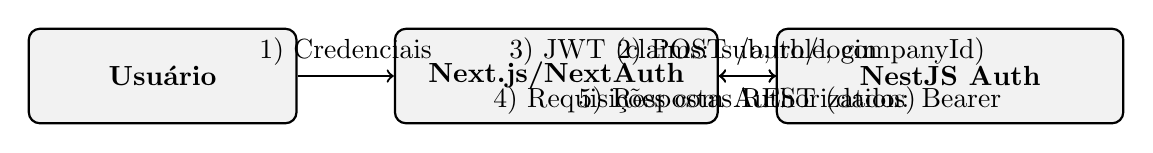
\begin{tikzpicture}
  % Nós
  \node[draw, rounded corners, thick, fill=gray!10, minimum width=3.4cm, minimum height=1.2cm] (user) at (0,0) {\textbf{Usuário}};
  \node[draw, rounded corners, thick, fill=gray!10, minimum width=4.1cm, minimum height=1.2cm] (fe) at (5,0) {\textbf{Next.js/NextAuth}};
  \node[draw, rounded corners, thick, fill=gray!10, minimum width=4.4cm, minimum height=1.2cm] (be) at (10,0) {\textbf{NestJS Auth}};

  % Passos
  \draw[->, thick] (user) -- node[above]{1) Credenciais} (fe);
  \draw[->, thick] (fe) -- node[above]{2) POST /auth/login} (be);
  \draw[->, thick] (be) -- node[above]{3) JWT (claims: sub, role, companyId)} (fe);
  \draw[->, thick] (fe) -- node[below]{4) Requisições com Authorization: Bearer} (be);
  \draw[->, thick] (be) -- node[below]{5) Respostas REST (dados)} (fe);
\end{tikzpicture}
\caption{Fluxo simplificado de autenticação e consumo da API.}
\label{fig:fluxo-auth}
\end{figure}

\section{Arquitetura do Frontend}
O frontend emprega Next.js~15 (React~19) com App Router, compondo páginas e layouts por segmentos de negócio (\texttt{/dashboard/[company]/...}). Destacam-se:

\begin{itemize}
  \item \textbf{Sessão e Contexto}: NextAuth com \textit{credentials provider}; o token JWT é persistido na sessão e exposto a componentes via \texttt{useSession} e por um contexto de autenticação.
  \item \textbf{Serviços de API}: um cliente consolidado (\texttt{api.service.ts}) monta a URL base (\texttt{NEXT\_PUBLIC\_API\_URL}), anexa o token \texttt{Bearer}, trata erros e respostas padronizadas e redireciona para login em caso de 401.
  \item \textbf{Camada de UI}: biblioteca de componentes com Radix UI e Tailwind CSS, compondo tabelas, diálogos e formulários tipados com React Hook Form e Zod.
  \item \textbf{Mapas e Geografia}: Leaflet/React-Leaflet para visualização e edição de rotas e paradas (componentes de mapa, formulários e tabelas integrados).
  \item \textbf{Organização por Domínio}: páginas e componentes agrupados por recursos (empresas, motoristas, veículos, rotas, viagens, bilhetes) favorecem coesão e evolução incremental.
\end{itemize}

Essa arquitetura promove: (i) separação de preocupações, (ii) segurança com \textit{JWT} e papéis, (iii) multiempresa por chave de escopo e (iv) escalabilidade via modularização e tipagem estática de ponta a ponta.
